

\tikzset{every picture/.style={line width=0.75pt}} %set default line width to 0.75pt        

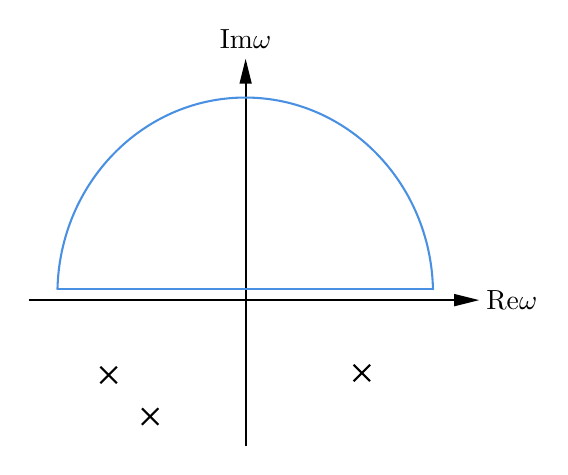
\begin{tikzpicture}[x=0.75pt,y=0.75pt,yscale=-1,xscale=1]
%uncomment if require: \path (0,300); %set diagram left start at 0, and has height of 300

%Straight Lines [id:da04442762060226202] 
\draw [color={rgb, 255:red, 0; green, 0; blue, 0 }  ,draw opacity=1 ]   (147.5,171.58) -- (362.5,171.58) ;
\draw [shift={(364.5,171.58)}, rotate = 180] [fill={rgb, 255:red, 0; green, 0; blue, 0 }  ,fill opacity=1 ][line width=0.08]  [draw opacity=0] (12,-3) -- (0,0) -- (12,3) -- cycle    ;

%Straight Lines [id:da8756241508108107] 
\draw [color={rgb, 255:red, 0; green, 0; blue, 0 }  ,draw opacity=1 ]   (252,241.83) -- (252,57.33) ;
\draw [shift={(252,55.33)}, rotate = 90] [fill={rgb, 255:red, 0; green, 0; blue, 0 }  ,fill opacity=1 ][line width=0.08]  [draw opacity=0] (12,-3) -- (0,0) -- (12,3) -- cycle    ;

%Shape: Arc [id:dp8470042201654997] 
\draw  [draw opacity=0] (161.35,166.51) .. controls (162.43,115.4) and (202.26,74.21) .. (251.42,73.98) .. controls (300.83,73.76) and (341.17,115.01) .. (342.28,166.47) -- (251.82,168.64) -- cycle ; \draw  [color={rgb, 255:red, 74; green, 144; blue, 226 }  ,draw opacity=1 ] (161.35,166.51) .. controls (162.43,115.4) and (202.26,74.21) .. (251.42,73.98) .. controls (300.83,73.76) and (341.17,115.01) .. (342.28,166.47) ;
%Straight Lines [id:da485580862989043] 
\draw [color={rgb, 255:red, 74; green, 144; blue, 226 }  ,draw opacity=1 ]   (161.35,166.42) -- (342.56,166.42) ;
%Straight Lines [id:da8631061251091796] 
\draw    (186,207.67) ;
\draw [shift={(186,207.67)}, rotate = 45] [color={rgb, 255:red, 0; green, 0; blue, 0 }  ][line width=0.75]    (-5.59,0) -- (5.59,0)(0,5.59) -- (0,-5.59)   ;
%Straight Lines [id:da042090732981503454] 
\draw    (206,227.67) ;
\draw [shift={(206,227.67)}, rotate = 45] [color={rgb, 255:red, 0; green, 0; blue, 0 }  ][line width=0.75]    (-5.59,0) -- (5.59,0)(0,5.59) -- (0,-5.59)   ;
%Straight Lines [id:da547231349279578] 
\draw    (308,206.67) ;
\draw [shift={(308,206.67)}, rotate = 45] [color={rgb, 255:red, 0; green, 0; blue, 0 }  ][line width=0.75]    (-5.59,0) -- (5.59,0)(0,5.59) -- (0,-5.59)   ;

% Text Node
\draw (252,51.93) node [anchor=south] [inner sep=0.75pt]    {$\mathrm{Im} \omega $};
% Text Node
\draw (366.5,171.58) node [anchor=west] [inner sep=0.75pt]    {$\mathrm{Re} \omega $};


\end{tikzpicture}
